\mysection{}{Vorüberlegungen} \label{sec:Vorueberlegungen}

Um die Fragestellung realistisch umsetzen zu können ist es nötig, schon vorab Entscheidungen über Richtung und Umfang des Projekts zu treffen.

\subsection{Plugin-Umfang}
Es soll Entwicklern mit Uniplug möglich sein, ohne Kenntnis der nativen Programmierschnittstelle der jeweiligen 3D-Software, Plugins zu entwickeln. Hier könnten im Voraus Einschränkungen getroffen werden um die Entwicklung zu vereinfachen. Zum Beispiel wäre es möglich sich auf die Erzeugung von Geometrie zu beschränken.

\subsection{Plugin-Arten}
Um abschätzen zu können, welche Funktionen in das Uniplug mit aufgenommen werden müssen, muss vorher überlegt werden, welche Plugin-Arten ein Plugin-Entwickler eventuell programmieren möchte. Ein 3D-Grafikprogramm ist recht vielseitig und bringt daher viele Möglichkeiten für Erweiterungen mit sich. Hierzu zählen sicherlich Import und Export Möglichkeiten für individuelle Datentypen. Dies ist besonders in Hinblick auf FUSEE interessant. Hierbei ist wichtig zu überlegen, welche Daten in der exportierten Datei gespeichert werden sollen und in welchem Format sie weitergegeben werden müssen. Dies hängt natürlich von den Programmen ab, die diese weiterverwenden sollen. Hier sind nicht nur Objektgrößen wichtig, sondern eventuell auch Hierarchiebäume, Lichtberechnungen, Animationen und vieles mehr.

Weitere Plugins könnten 3D-Programme durch verschiedene Funktionen erweitern. Hier wären neue Mesh-Operationen, neue Standardobjekte oder andere Zugriffe auf den Szenengraph denkbar. Interessant könnten weitere Parameter oder Objekttypen sein.

Bei der Überlegung muss immer bedacht werden, dass Daten in verschiedenen Programmen unterschiedlich gespeichert und gehandhabt werden. Allein die Liste der Projektgruppe hat eine riesige Anzahl an möglichen Plugin-Funktionen, die ihre eigenen Komplikationen mit sich bringen. Hier wurde schnell klar, dass nicht alle Funktionen gleich berücksichtigt werden können.
 
\subsection{Plugin-Aufbau}
Vorab wurden zwei Ansätze für den Aufbau von Uniplug evaluiert. Außer der schon teilweise beschriebenen kompletten und am besten automatisierte Übersetzung der Programmierschnittstelle, gibt es noch die Möglichkeit nativ für die jeweilige Software ein Plugin zu entwickeln, das dann die zu übersetzende Schnittstelle zu Uniplug bildet und somit schon einen ersten Schritt zur Normalisierung und logischen Übersetzung bietet. Weitere Informationen zu den einzelnen Verfahren finden sich in \ref{sec:header}.

\subsection{Entscheidungen}
Die Entscheidung fiel auf eine möglichst vollständige Übersetzung ohne Zwischenschritt über ein Plugin. Dieser Ansatz bietet aber bei Erfolg einen wesentlich direkteren und auch komfortableren Zugriff auf Seiten von Uniplug, da jegliche logische Konvertierung im Rahmen von \CS direkt als Teil von Uniplug erfolgen kann.

\begin{figure}[htbp]
\center
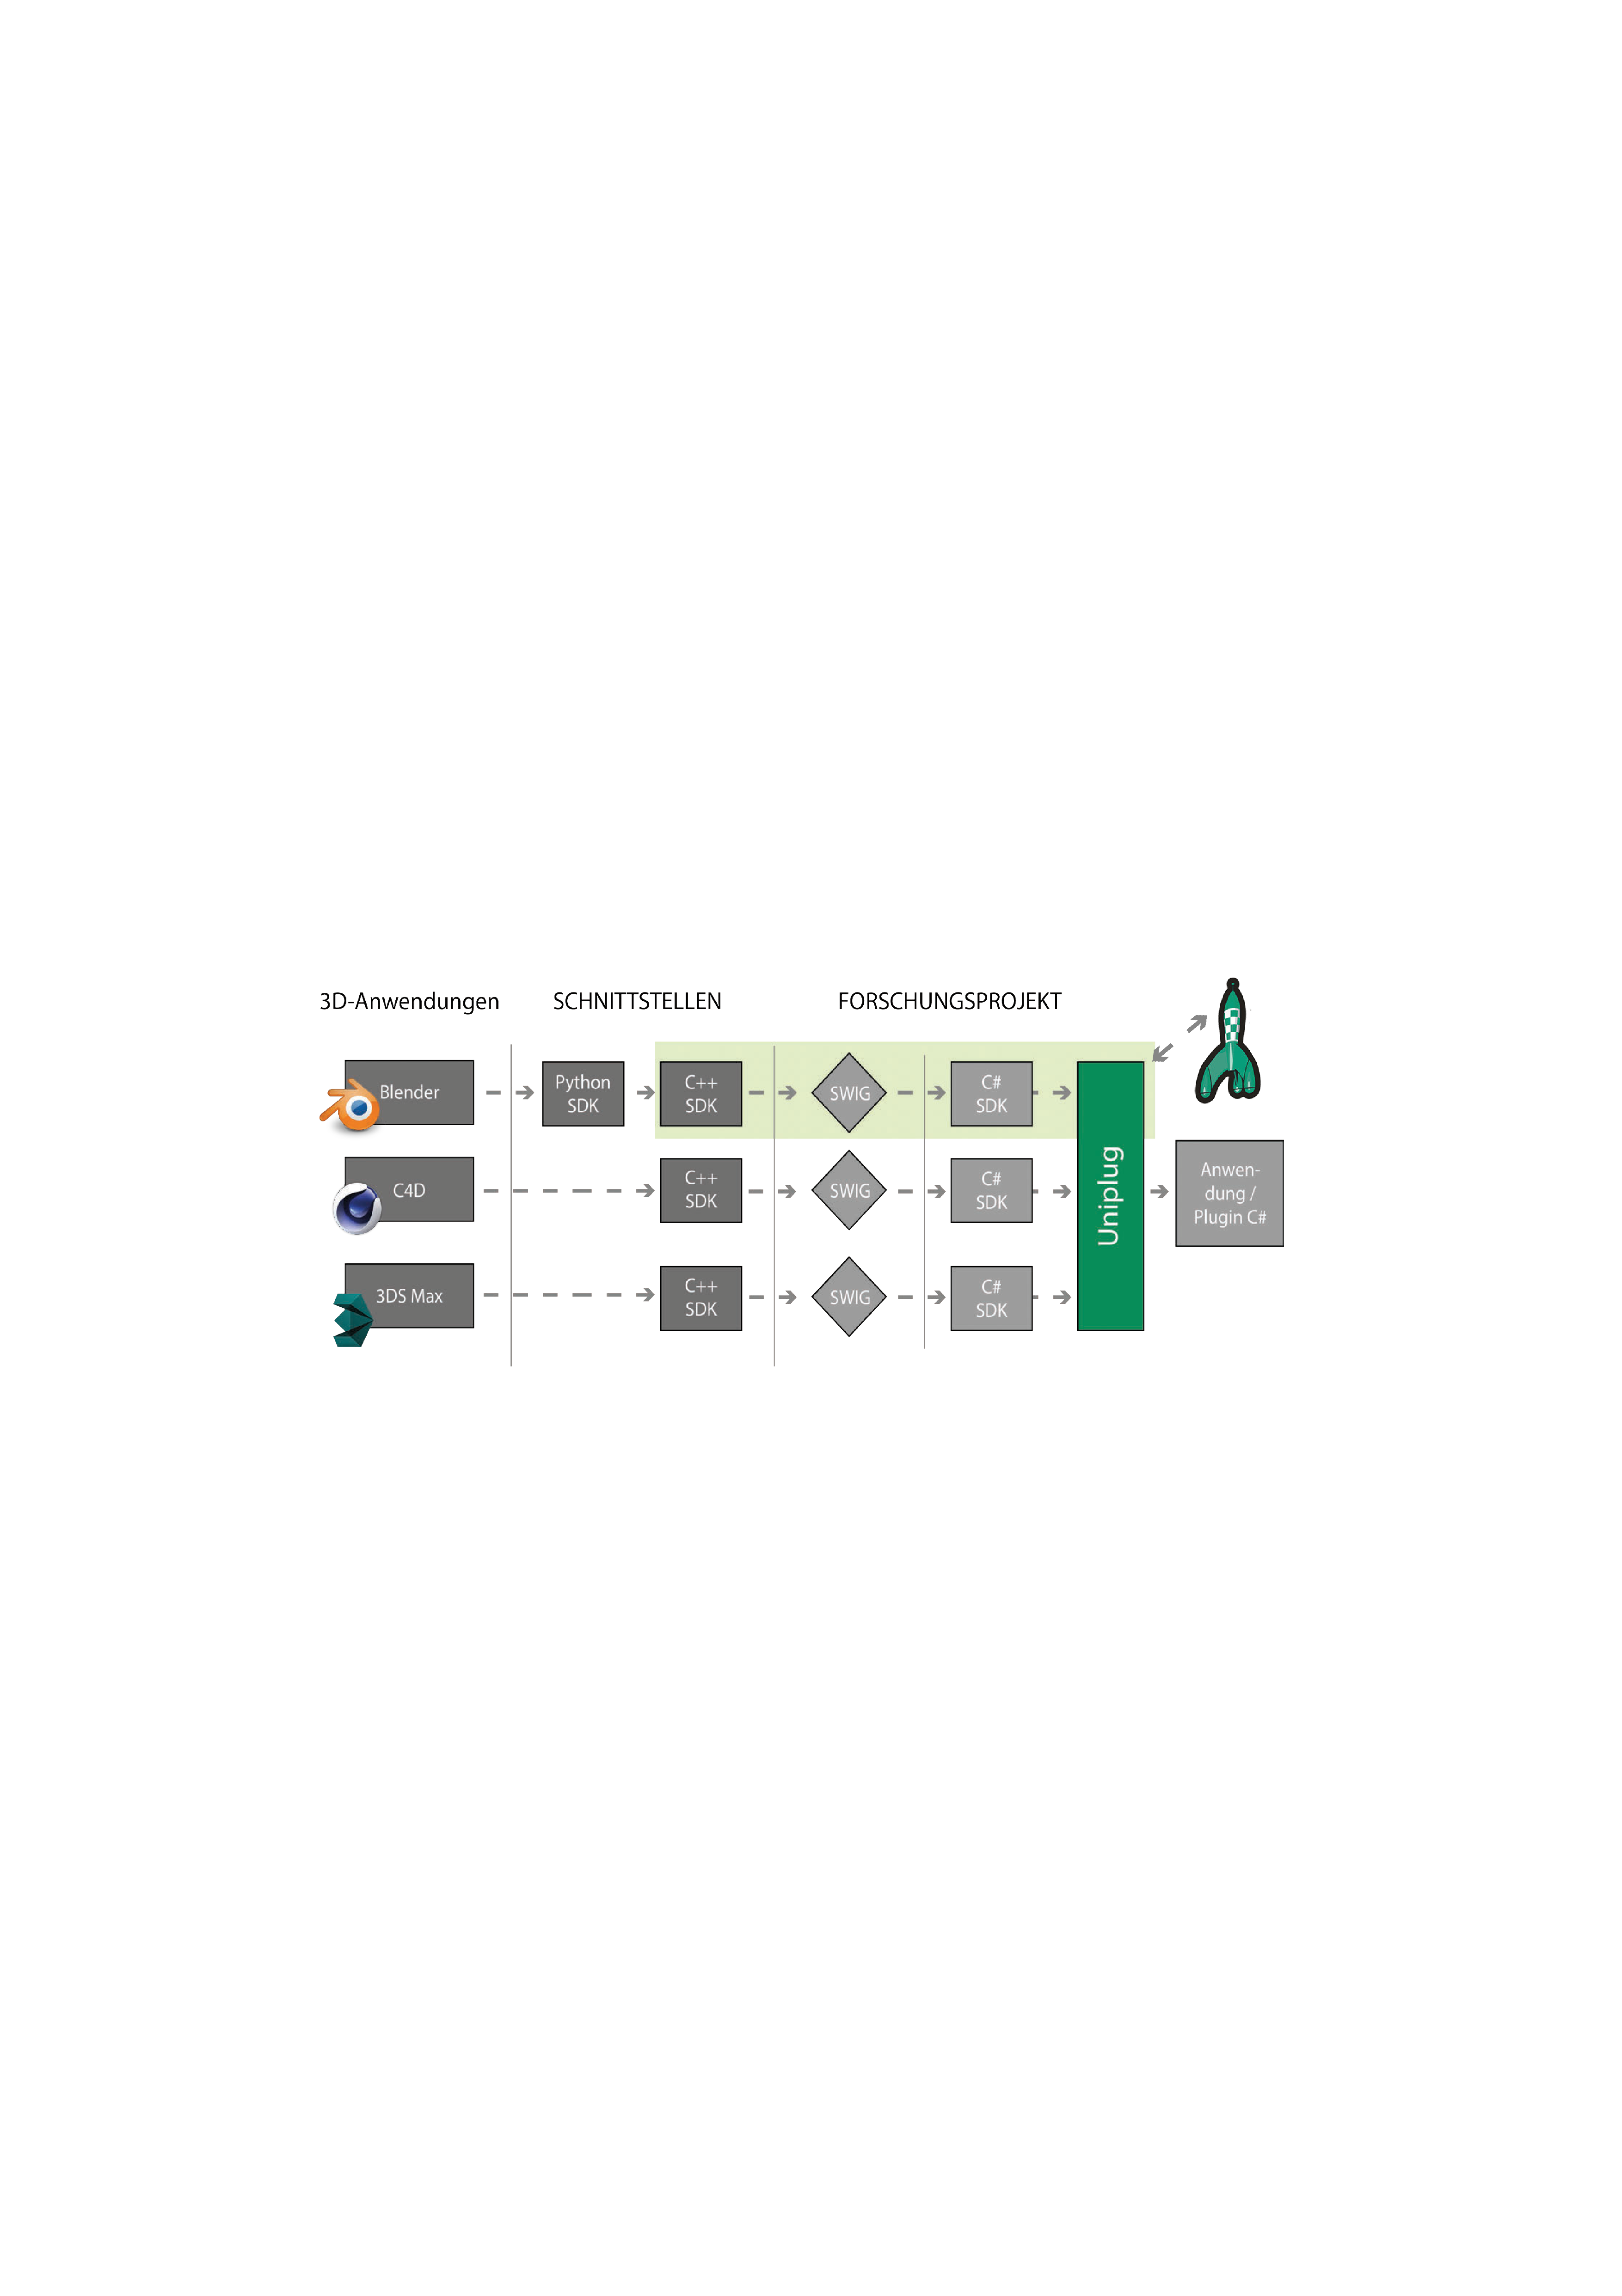
\includegraphics[width=1\textwidth]{images/aufbau}
\caption{Schematische Darstellung des Aufbaus}
\label{fig:aufbau}
\end{figure}